\section{Modello CPSO e semantiche di esecuzione}
\label{sec:model}

\subsection{Formulazione}
\label{subsec:cpso-original-formulation}

Il Continuous Particle Swarm Optimization (CPSO)~\citep{orlando2020analytic} introduce una descrizione continua del moto delle particelle a partire dal modello discreto del Particle Swarm Optimization (PSO). Si consideri uno sciame composto da $N_p$ particelle in uno spazio di ricerca di dimensione $n$. La posizione e la velocit\`a della particella $i$ al passo $\lambda$ sono indicate rispettivamente con $p_i^\lambda$ e $v_i^\lambda$, mentre $p_{ib}$ e $p_{gb}$ rappresentano la migliore posizione individuale e quella globale. L'aggiornamento discreto \`e definito da
\begin{equation}
 p_i^{\lambda+1}=p_i^\lambda+v_i^{\lambda+1},
 \label{eq:or-discrete-position}
\end{equation}
\begin{equation}
 v_i^{\lambda+1}=\mu v_i^\lambda
 +c_c r_1(p_{ib}-p_i^\lambda)
 +c_s r_2(p_{gb}-p_i^\lambda),
 \label{eq:or-discrete-velocity}
\end{equation}
dove $c_c$ e $c_s$ sono i coefficienti cognitivo e sociale, $r_1,r_2\in[0,1]$ sono variabili casuali e $\mu$ \`e il peso d'inerzia, che varia linearmente secondo
\begin{equation}
 \mu=\mu_{\max}-\frac{\mu_{\max}-\mu_{\min}}{\lambda_{\max}}\lambda.
 \label{eq:or-inertia}
\end{equation}
Sottraendo $v_i^\lambda$ ai due membri dell'equazione della velocit\`a si ottiene
\begin{equation}
\begin{aligned}
 v_i^{\lambda+1}-v_i^\lambda
 ={}&(\mu-1)v_i^\lambda+c_c r_1(p_{ib}-p_i^\lambda)\\
 &+c_s r_2(p_{gb}-p_i^\lambda).
\end{aligned}
\label{eq:or-velocity-difference}
\end{equation}

Interpretando l'incremento temporale unitario della formulazione discreta come un intervallo infinitesimo $\delta t$ e considerando il limite $\delta t\to0$, il quoziente incrementale della velocit\`a conduce a un'equazione differenziale del secondo ordine. Omettendo l'indice della particella, si introduce il vettore posizione $p(t)=[x_1(t),\ldots,x_n(t)]$. Il corrispondente problema di Cauchy \`e
\begin{equation}
\begin{cases}
 \ddot p(t)+(1-\mu(t))\dot p(t)
 +(c_c r_1(t)+c_s r_2(t))p(t)=f(t),\\
 p(0)=p_0,\\
 \dot p(0)=\dot p_0,
\end{cases}
\label{eq:or-cauchy}
\end{equation}
con termine forzante
\begin{equation}
 f(t)=c_c r_1(t)p_{ib}(t)+c_s r_2(t)p_{gb}(t).
 \label{eq:or-force-time}
\end{equation}
La funzione obiettivo da minimizzare sar\`a indicata con $J$, riservando il simbolo $f$ al termine forzante dell'equazione differenziale.

Introducendo la pulsazione naturale $\omega:[0,T]\to[0,+\infty)$ e il rapporto di smorzamento $\zeta:[0,T]\to[0,1]$ mediante
\begin{equation}
\begin{cases}
 2\zeta(t)\omega(t)=1-\mu(t),\\
 \omega^2(t)=c_c r_1(t)+c_s r_2(t),
\end{cases}
\label{eq:or-oscillator-parameters}
\end{equation}
il problema assume la forma di un oscillatore armonico smorzato:
\begin{equation}
\begin{cases}
 \ddot p(t)+2\zeta(t)\omega(t)\dot p(t)
 +\omega^2(t)p(t)=f(t),\\
 p(0)=p_0,\\
 \dot p(0)=\dot p_0.
\end{cases}
\label{eq:or-oscillator}
\end{equation}

Per ricavare la soluzione analitica, l'intervallo di integrazione $[0,T]$ viene suddiviso in $N$ sottointervalli di ampiezza $dt=T/N$. In ciascuno di essi si assumono costanti la pulsazione e il rapporto di smorzamento:
\begin{equation}
\begin{cases}
 \omega(t)=\omega_k,\\
 \zeta(t)=\zeta_k,
\end{cases}
\qquad t\in[kdt,(k+1)dt],\quad k=0,\ldots,N-1.
\label{eq:or-piecewise}
\end{equation}
Si ottiene cos\`i, su ogni sottointervallo, il problema lineare a coefficienti costanti
\begin{equation}
\begin{cases}
 \ddot p(t)+2\zeta_k\omega_k\dot p(t)+\omega_k^2p(t)=f_k,\\
 p(kdt)=p_k,\\
 \dot p(kdt)=\dot p_k,
\end{cases}
\label{eq:or-local}
\end{equation}
con
\begin{equation}
 f_k=c_c p_{ib}(kdt)+c_s p_{gb}(kdt).
 \label{eq:or-force-printed}
\end{equation}
La soluzione sul $k$-esimo sottointervallo \`e indicata con $p_{[kdt,(k+1)dt]}(t)$. Le condizioni iniziali del sottointervallo successivo sono assegnate mediante il raccordo
\begin{equation}
\begin{cases}
 p_k=p_{[(k-1)dt,kdt]}(kdt),\\
 \dot p_k=\dot p_{[(k-1)dt,kdt]}(kdt),
\end{cases}
\qquad k=1,\ldots,N-1,
\label{eq:or-matching}
\end{equation}
in modo da costruire la soluzione a tratti sull'intero intervallo di integrazione:
\begin{equation}
 p(t)=\bigcup_{k=0}^{N-1}p_{[kdt,(k+1)dt]}(t).
 \label{eq:or-piecewise-solution}
\end{equation}
La propagazione di posizione e velocit\`a deriva pertanto dalla soluzione analitica di ciascun problema locale e dall'applicazione successiva delle condizioni di raccordo~\citep{orlando2020analytic}.

\subsection{Notazione per l'estensione parallela}
\label{subsec:cpso-implementation}

Per l'estensione parallela si usano $N_p$ per la cardinalit\`a dello sciame, $D=n$ per la dimensione dello spazio di ricerca, $K$ per il numero di aggiornamenti e $dt$ per l'ampiezza del sottointervallo temporale. La posizione e la velocit\`a della particella $i$ all'inizio del sottointervallo $k$ sono indicate con $\bm x_i^k$ e $\bm v_i^k$. Si introducono inoltre il migliore individuale $\bm p_i^k$ e il leader sociale $\bm s_i^k$, coincidente con il migliore globale nel caso di comunicazione globale e con il migliore del vicinato nelle estensioni topologiche.

Ponendo
\begin{equation}
 a_i^k=c_c r_{1,i}^k,\qquad
 b_i^k=c_s r_{2,i}^k,\qquad
 q_i^k=a_i^k+b_i^k,
 \label{eq:cpso-weights}
\end{equation}
la corrispondente dinamica continua su un sottointervallo assume la forma
\begin{equation}
 \ddot{\bm x}_i+(1-\mu_k)\dot{\bm x}_i
 +q_i^k\bm x_i=a_i^k\bm p_i^k+b_i^k\bm s_i^k.
 \label{eq:cpso-model}
\end{equation}
Tale notazione consente di descrivere una stessa dinamica con diverse strutture d'interazione tra particelle, mantenendo distinto il modello continuo di base dalle scelte proprie della sua estensione parallela. La soluzione locale dell'Eq.~\eqref{eq:cpso-model} è riportata in Appendice~\ref{app:dynamics}.

\subsection{Modalità di esecuzione}
La Tabella~\ref{tab:execution-modes} distingue le tre modalità sincrone. A inizio generazione, ciascuna modalità fissa i migliori individuali e i leader sociali da cui partono tutte le proposte. I valori obiettivo sono raccolti prima di aggiornare i migliori in ordine di particella. Con un obiettivo deterministico e condizioni iniziali, coefficienti casuali e aritmetica comuni, due esecuzioni che partono dallo stesso stato calcolano le stesse proposte e raggiungono lo stesso stato alla generazione successiva. Nella modalità asincrona, l'informazione resa disponibile al completamento delle singole valutazioni può influenzare gli aggiornamenti successivi.

\begin{table*}[!tbp]
\centering\small
\caption{Modalità sincrone del CPSO e ripartizione del lavoro in ciascuna generazione.}
\label{tab:execution-modes}
\begin{tabularx}{\textwidth}{@{}p{2.7cm}X X p{3.25cm}@{}}
\toprule
Modalità & Distribuzione del lavoro & Disponibilità del leader & Ruolo nel confronto \\
\midrule
Seriale & Inizializzazione, propagazione e valutazioni su un solo thread. & Fissato a inizio generazione. & Riferimento seriale. \\
Master--slave & Valutazioni distribuite. Propagazione e aggiornamento dei migliori seriali. & Fissato a inizio generazione. & Parallelismo delle valutazioni. \\
Particle-parallel & Inizializzazione, propagazione e valutazioni distribuite. Aggiornamento ordinato dei migliori. & Fissato a inizio generazione. & Parallelismo per particella. \\
\bottomrule
\end{tabularx}
\end{table*}

La valutazione della popolazione iniziale e $K$ aggiornamenti completi per particella richiedono
\begin{equation}
 B_{\mathrm{FE}}=N_p(K+1)
 \label{eq:fe-budget}
\end{equation}
valutazioni della funzione obiettivo (FE). Nei confronti con le varianti PSO si contabilizzano le valutazioni effettive, poiché alcuni metodi rivalutano solo una parte dello sciame a ciascuna iterazione.

\subsection{Topologie sociali}
Il grafo sociale definisce l'insieme di particelle da cui ciascuna può apprendere. I grafi sono non orientati e restano fissi durante l'esecuzione. Il vicinato comprende la particella stessa e il suo leader è il migliore tra i punti personali dei vicini. Le otto configurazioni corrispondono a sette famiglie, con due livelli di densità per il grafo casuale. La Figura~\ref{fig:topology-schematics} illustra i collegamenti e la Tabella~\ref{tab:app-graphs} ne specifica la costruzione. Global e Random-8 sono i vicinati impiegati nelle campagne finali di cui alla Sezione~\ref{sec:exp}.

\begin{figure*}[tbp]
\centering
\setlength{\tabcolsep}{3pt}
\begin{tabular}{cccc}
\begin{minipage}[t]{0.22\textwidth}\centering
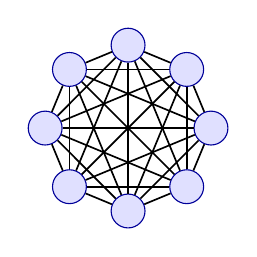
\begin{tikzpicture}[scale=0.78, every node/.style={circle,draw,fill=white,inner sep=1.3pt,minimum size=4.3mm,font=\scriptsize},
edge/.style={line width=0.6pt}, hl/.style={fill=blue!12,draw=blue!60!black}]
  \foreach \i/\ang in {1/90,2/45,3/0,4/315,5/270,6/225,7/180,8/135}{
    \node[hl] (n\i) at (\ang:1.35) {};
  }
  \foreach \i/\j in {1/2,1/3,1/4,1/5,1/6,1/7,1/8,2/3,2/4,2/5,2/6,2/7,2/8,3/4,3/5,3/6,3/7,3/8,4/5,4/6,4/7,4/8,5/6,5/7,5/8,6/7,6/8,7/8}{
    \draw[edge] (n\i)--(n\j);
  }
\end{tikzpicture}
\par\vspace{1mm}\scriptsize \textbf{(a) Global-best}
\end{minipage}
&
\begin{minipage}[t]{0.22\textwidth}\centering
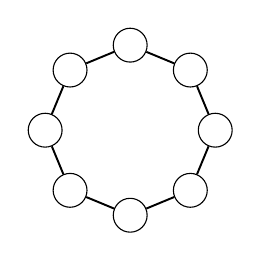
\begin{tikzpicture}[scale=0.8, every node/.style={circle,draw,fill=white,inner sep=1.3pt,minimum size=4.3mm,font=\scriptsize}, edge/.style={line width=0.7pt}]
  \foreach \i/\ang in {1/90,2/45,3/0,4/315,5/270,6/225,7/180,8/135}{
    \node (n\i) at (\ang:1.35) {};
  }
  \foreach \i/\j in {1/2,2/3,3/4,4/5,5/6,6/7,7/8,8/1}{\draw[edge] (n\i)--(n\j);}  
\end{tikzpicture}
\par\vspace{1mm}\scriptsize \textbf{(b) Ring}
\end{minipage}
&
\begin{minipage}[t]{0.22\textwidth}\centering
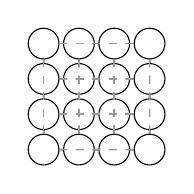
\begin{tikzpicture}[scale=0.66, every node/.style={circle,draw,fill=white,inner sep=1.0pt,minimum size=3.9mm,font=\scriptsize}, edge/.style={line width=0.6pt}, wrap/.style={line width=0.6pt,dashed,gray!80}]
  \foreach \r in {1,2,3,4}{
    \foreach \c in {1,2,3,4}{
      \pgfmathtruncatemacro{\id}{4*(\r-1)+\c}
      \node (n\id) at (0.68*\c, -0.68*\r) {};
    }
  }
  \foreach \r in {1,2,3,4}{
    \foreach \c in {1,2,3,4}{
      \pgfmathtruncatemacro{\cn}{mod(\c,4)+1}
      \pgfmathtruncatemacro{\a}{4*(\r-1)+\c}
      \pgfmathtruncatemacro{\b}{4*(\r-1)+\cn}
      \ifnum\c<4 \draw[edge] (n\a)--(n\b); \else \draw[wrap] (n\a)--(n\b); \fi
    }
  }
  \foreach \c in {1,2,3,4}{
    \foreach \r in {1,2,3,4}{
      \pgfmathtruncatemacro{\rn}{mod(\r,4)+1}
      \pgfmathtruncatemacro{\a}{4*(\r-1)+\c}
      \pgfmathtruncatemacro{\b}{4*(\rn-1)+\c}
      \ifnum\r<4 \draw[edge] (n\a)--(n\b); \else \draw[wrap] (n\a)--(n\b); \fi
    }
  }
\end{tikzpicture}
\par\vspace{1mm}\scriptsize \textbf{(c) Griglia von Neumann toroidale}
\end{minipage}
&
\begin{minipage}[t]{0.22\textwidth}\centering
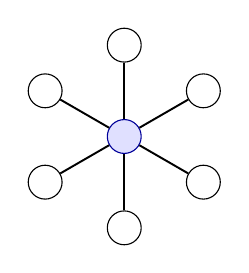
\begin{tikzpicture}[scale=0.8, every node/.style={circle,draw,fill=white,inner sep=1.3pt,minimum size=4.3mm,font=\scriptsize}, edge/.style={line width=0.7pt}, hub/.style={fill=blue!12,draw=blue!60!black}]
  \node[hub] (c) at (0,0) {};
  \foreach \i/\ang in {1/90,2/30,3/330,4/270,5/210,6/150}{
    \node (n\i) at (\ang:1.45) {};
    \draw[edge] (c)--(n\i);
  }
\end{tikzpicture}
\par\vspace{1mm}\scriptsize \textbf{(d) Wheel nell'API (hub-and-spoke)}
\end{minipage}
\\[1.8ex]
\begin{minipage}[t]{0.22\textwidth}\centering
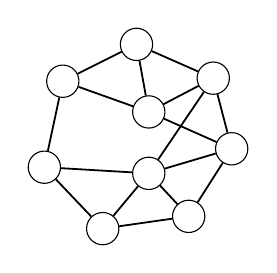
\begin{tikzpicture}[scale=0.78, every node/.style={circle,draw,fill=white,inner sep=1.1pt,minimum size=4.1mm,font=\scriptsize}, edge/.style={line width=0.65pt}]
  \foreach \i/\x/\y in {1/0/1.55,2/1.25/1.0,3/1.55/-0.15,4/0.85/-1.25,5/-0.55/-1.45,6/-1.5/-0.45,7/-1.2/0.95,8/0.2/0.45,9/0.2/-0.55}{
    \node (n\i) at (\x,\y) {};
  }
  \foreach \i/\j in {1/2,1/8,1/7,2/3,2/8,2/9,3/8,3/9,3/4,4/5,4/9,5/6,5/9,6/7,6/9,7/8}{\draw[edge] (n\i)--(n\j);}  
\end{tikzpicture}
\par\vspace{1mm}\scriptsize \textbf{(e) Random connessa, $k\approx4$}
\end{minipage}
&
\begin{minipage}[t]{0.22\textwidth}\centering
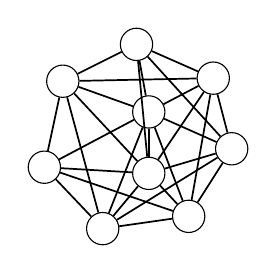
\begin{tikzpicture}[scale=0.78, every node/.style={circle,draw,fill=white,inner sep=1.1pt,minimum size=4.1mm,font=\scriptsize}, edge/.style={line width=0.62pt}]
  \foreach \i/\x/\y in {1/0/1.55,2/1.25/1.0,3/1.55/-0.15,4/0.85/-1.25,5/-0.55/-1.45,6/-1.5/-0.45,7/-1.2/0.95,8/0.2/0.45,9/0.2/-0.55}{
    \node (n\i) at (\x,\y) {};
  }
  \foreach \i/\j in {1/2,1/3,1/7,1/8,1/9,2/3,2/4,2/7,2/8,2/9,3/4,3/5,3/8,3/9,4/5,4/6,4/8,4/9,5/6,5/7,5/8,5/9,6/7,6/8,6/9,7/8,7/9,8/9}{\draw[edge] (n\i)--(n\j);}  
\end{tikzpicture}
\par\vspace{1mm}\scriptsize \textbf{(f) Random connessa, $k\approx8$}
\end{minipage}
&
\begin{minipage}[t]{0.22\textwidth}\centering
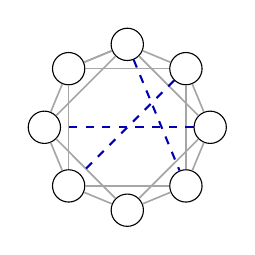
\begin{tikzpicture}[scale=0.78, every node/.style={circle,draw,fill=white,inner sep=1.1pt,minimum size=4.1mm,font=\scriptsize}, edge/.style={line width=0.6pt}, shortcut/.style={line width=0.75pt,blue!70!black,dashed}]
  \foreach \i/\ang in {1/90,2/45,3/0,4/315,5/270,6/225,7/180,8/135}{\node (n\i) at (\ang:1.35) {};}
  \foreach \i/\j in {1/2,2/3,3/4,4/5,5/6,6/7,7/8,8/1,1/8,1/3,2/4,3/5,4/6,5/7,6/8,7/1,8/2}{\draw[edge,gray!70] (n\i)--(n\j);} 
  \foreach \i/\j in {1/4,2/6,3/7}{\draw[shortcut] (n\i)--(n\j);}  
\end{tikzpicture}
\par\vspace{1mm}\scriptsize \textbf{(g) Small-world, $k=4$}
\end{minipage}
&
\begin{minipage}[t]{0.22\textwidth}\centering
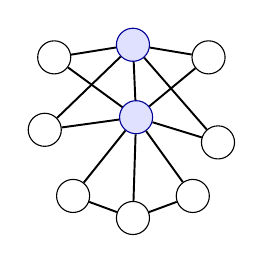
\begin{tikzpicture}[scale=0.8, every node/.style={circle,draw,fill=white,inner sep=1.1pt,minimum size=4.2mm,font=\scriptsize}, edge/.style={line width=0.7pt}, hub/.style={fill=blue!12,draw=blue!60!black}]
  \node[hub] (h1) at (0,1.2) {};
  \node[hub] (h2) at (0.05,0.05) {};
  \node (n3) at (-1.25,1.0) {};
  \node (n4) at (1.2,1.0) {};
  \node (n5) at (-1.4,-0.15) {};
  \node (n6) at (1.35,-0.35) {};
  \node (n7) at (-0.95,-1.2) {};
  \node (n8) at (0.95,-1.2) {};
  \node (n9) at (0,-1.55) {};
  \foreach \i/\j in {h1/h2,h1/n3,h1/n4,h1/n5,h1/n6,h2/n3,h2/n4,h2/n5,h2/n6,h2/n7,h2/n8,h2/n9,n7/n9,n8/n9}{\draw[edge] (\i)--(\j);}  
\end{tikzpicture}
\par\vspace{1mm}\scriptsize \textbf{(h) Scale-free, $k=4$}
\end{minipage}
\end{tabular}
\caption{Schemi TikZ delle otto topologie di comunicazione discusse nel manoscritto. I pannelli sono rappresentazioni qualitative della struttura del vicinato e non corrispondono alla dimensione reale dello sciame usata negli esperimenti. Per le topologie random, small-world e scale-free si mostrano realizzazioni esemplificative; la topologia \texttt{wheel} implementata nel codice coincide con una struttura hub-and-spoke, cio\`e una stella, e non con la wheel grafica standard dotata di anello periferico. Nella griglia von Neumann le linee tratteggiate indicano i collegamenti periodici della topologia toroidale.}
\label{fig:topology-schematics}
\end{figure*}
\begin{table*}[!tbp]
\centering\small
\caption{Regole di costruzione degli otto vicinati sociali. Il parametro $k$ dei grafi R4 e R8 controlla la densità di campionamento.}
\label{tab:app-graphs}
\begin{tabularx}{\textwidth}{@{}lX@{}}
\toprule
Vicinato & Collegamenti tra particelle \\
\midrule
Global & Ogni particella ha accesso al migliore dell'intero sciame. \\
Ring & Ogni nodo è collegato ai due adiacenti nell'anello. \\
Von Neumann & Quattro adiacenze ortogonali su una griglia toroidale. Con $N_p=64$ la griglia è $8\times 8$. \\
Stella & Un hub scelto casualmente è collegato a tutti gli altri nodi. \\
Random-4 (R4) & Archi Bernoulli con probabilità $4/(N_p-1)$. Eventuali componenti vengono unite mediante ponti. \\
Random-8 (R8) & Archi Bernoulli con probabilità $8/(N_p-1)$ e stessa regola di connessione. \\
Small-world & Anello di grado quattro con probabilità di ricollegamento $0.15$ per arco. \\
Scale-free & Attaccamento preferenziale con due archi per nuovo nodo, a partire da tre nodi interamente connessi. \\
\bottomrule
\end{tabularx}
\end{table*}
